\section{Anhang}

\subsection{Markierte Objekte aus unterschiedlichen Blickwinkeln}
\label{appendix:blickwinkel}
\begin{figure}[H]
	\centering
	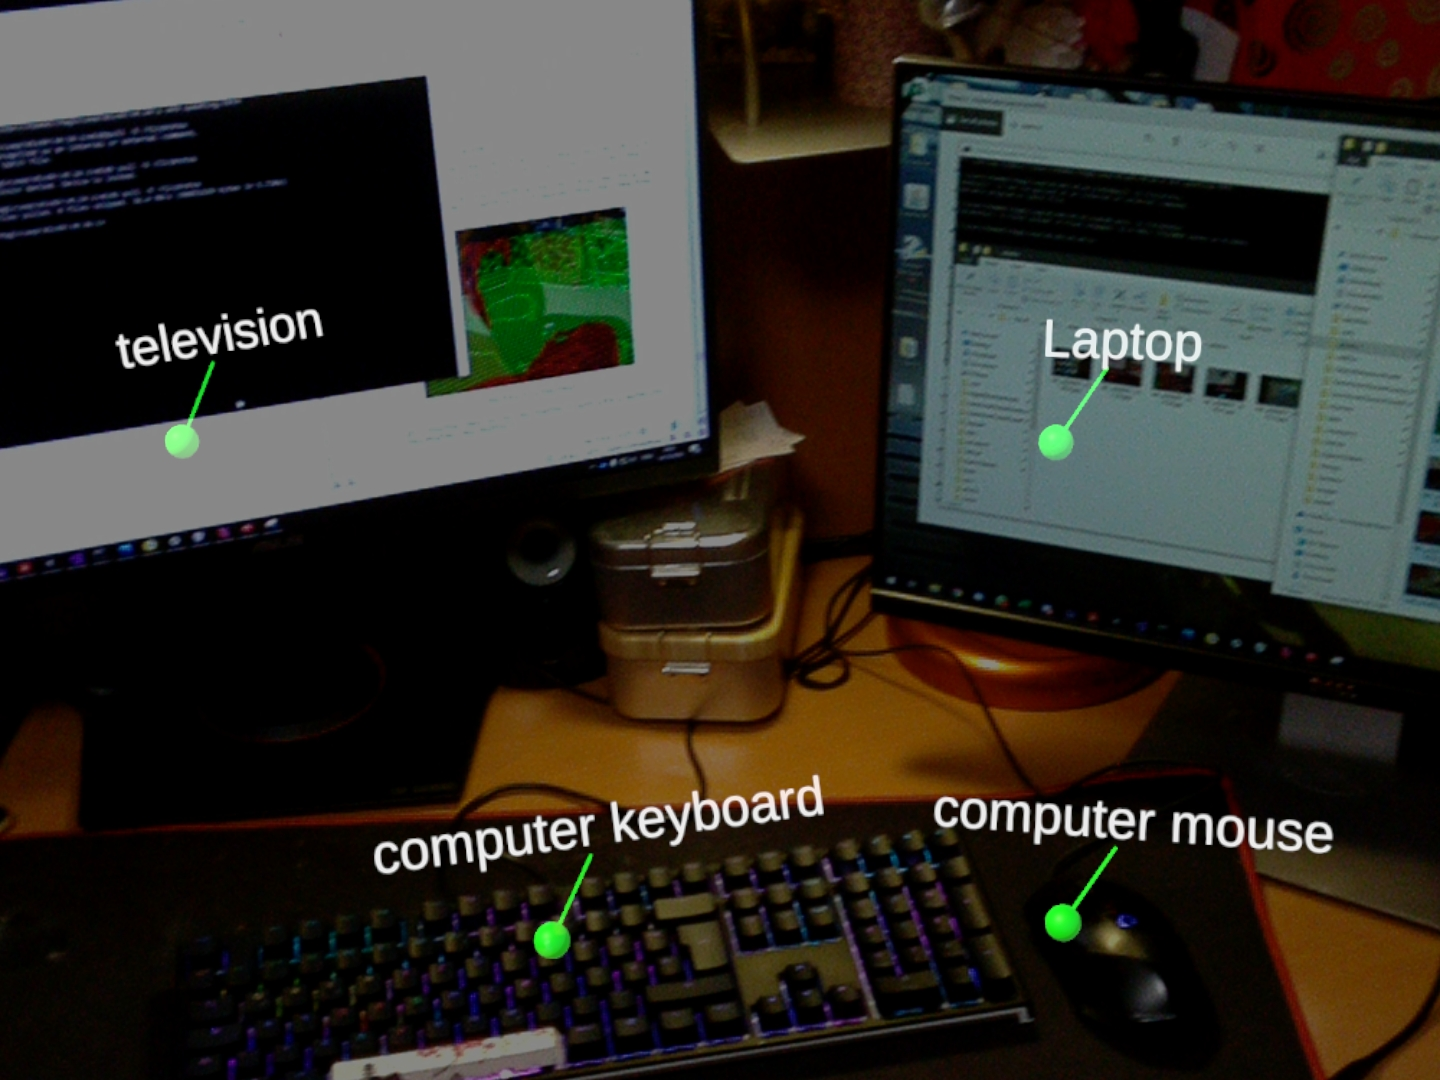
\includegraphics[width=0.8\textwidth]{images/ML_20201014_03.01.45.jpg}
	\caption[Objekte mit Label. Blickwinkel 1]{Objekte mit Label. Blickwinkel 1}
	\label{img:m1}
\end{figure}

\begin{figure}[H]
	\centering
	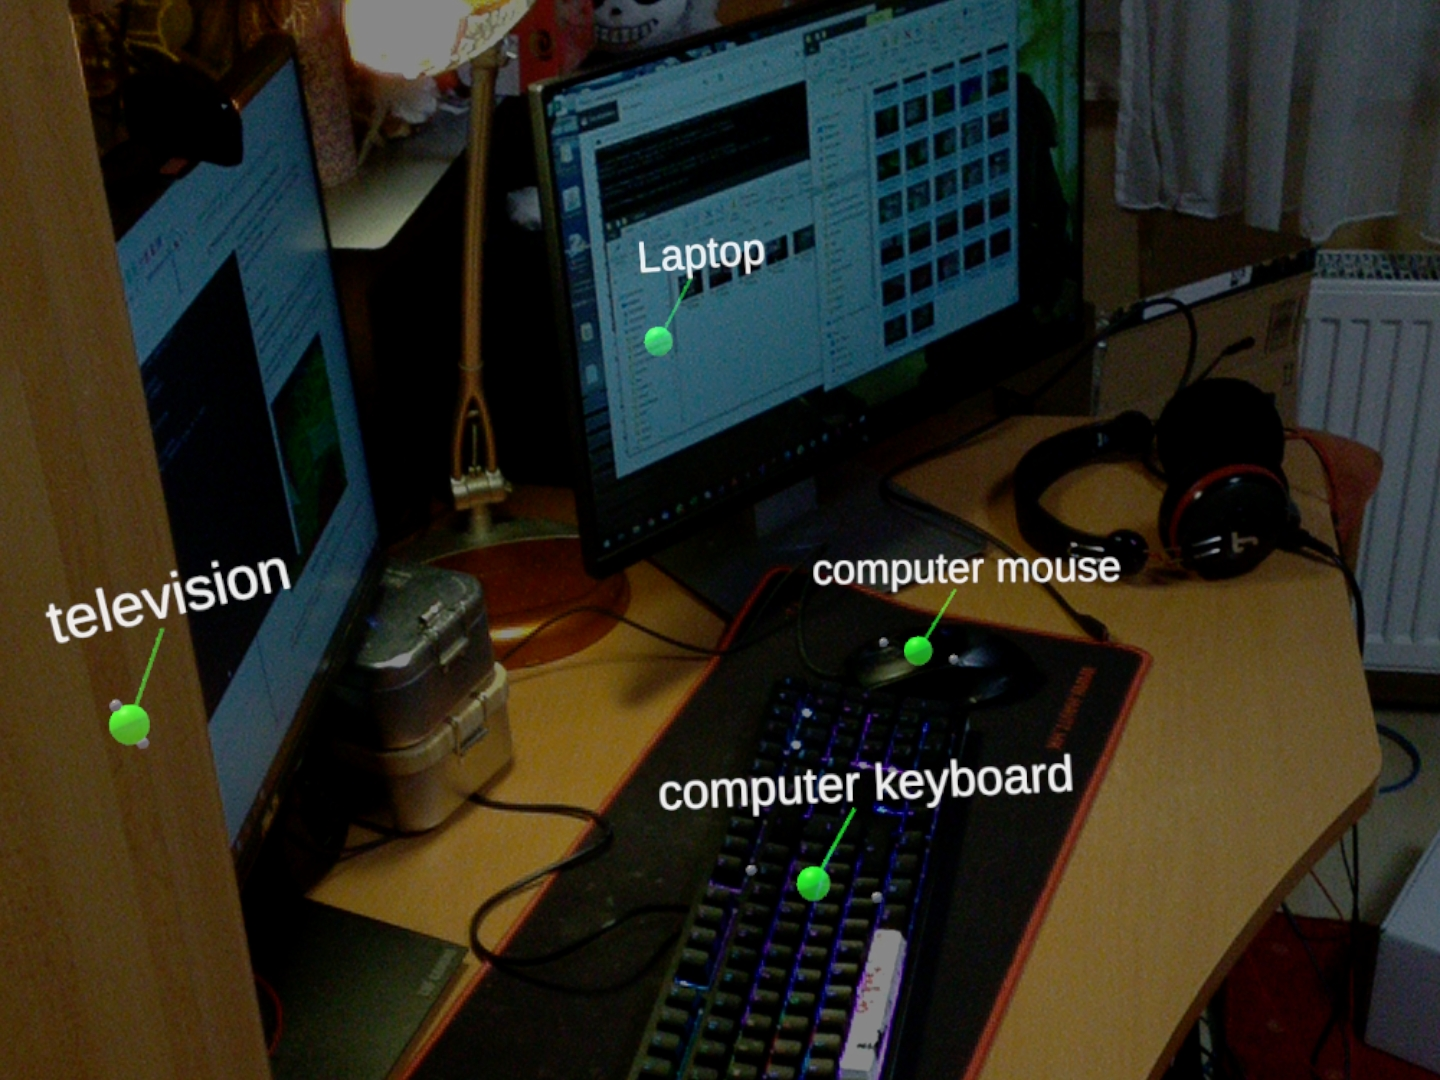
\includegraphics[width=0.8\textwidth]{images/ML_20201014_03.02.35.jpg}
	\caption[Objekte mit Label. Blickwinkel 2]{Blickwinkel 2}
	\label{img:m2}
\end{figure}
\begin{figure}[H]
	\centering
	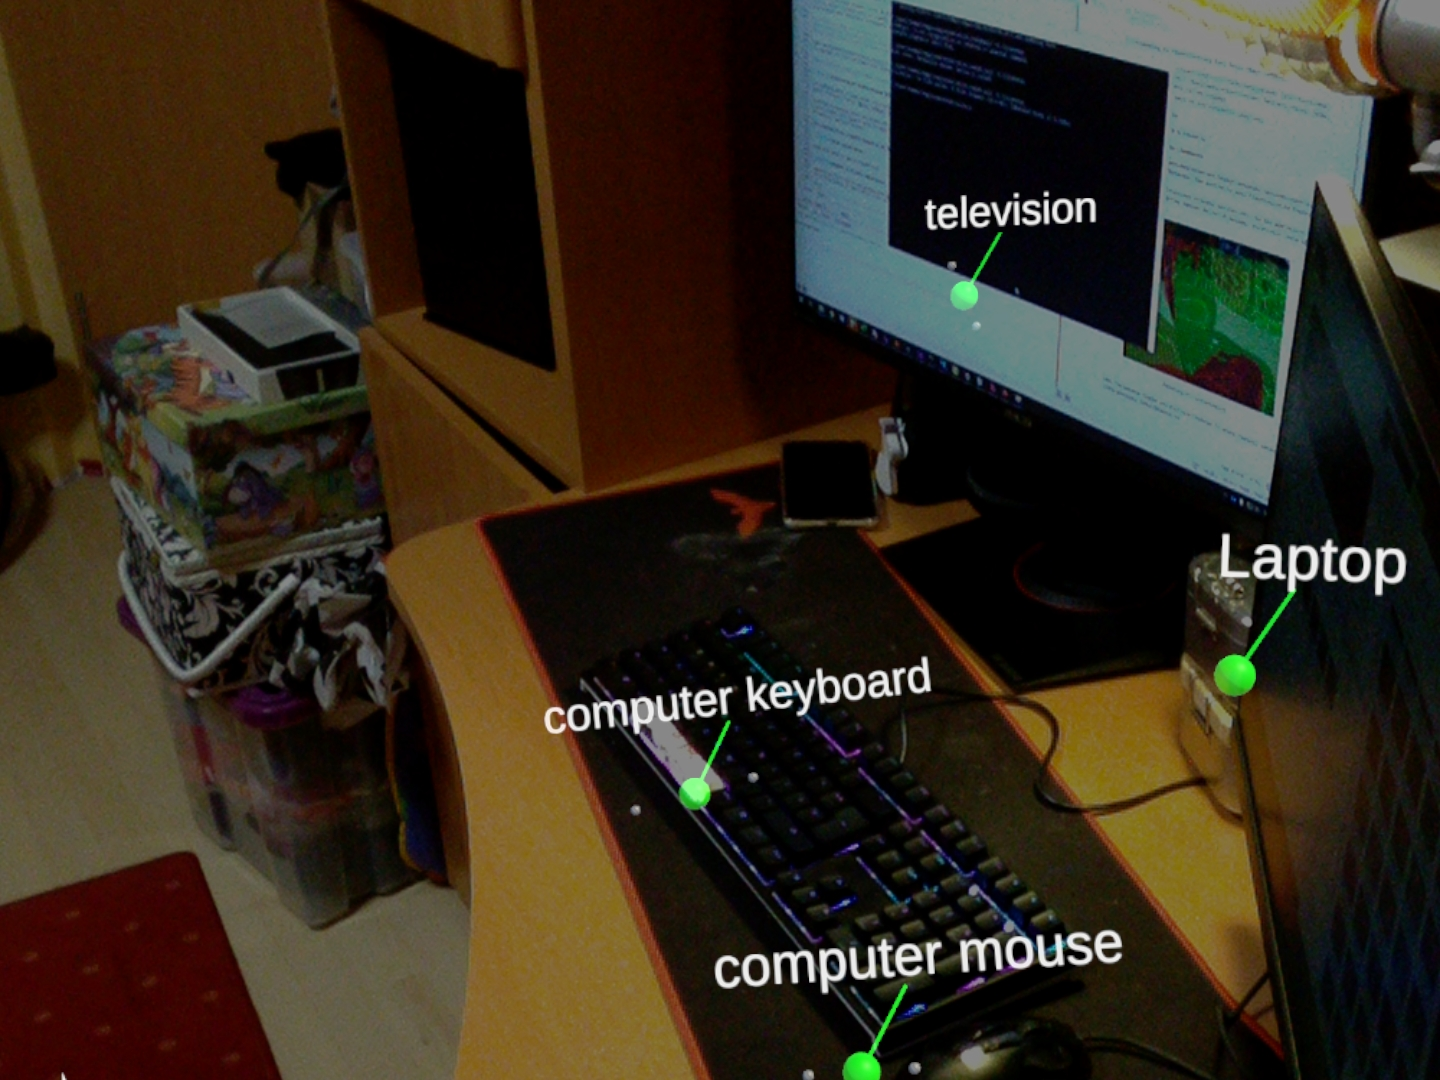
\includegraphics[width=0.8\textwidth]{images/ML_20201014_03.02.44.jpg}
	\caption[Objekte mit Label. Blickwinkel 3]{Blickwinkel 3}
	\label{img:m3}
\end{figure}

\subsection{Ausschnitt Traininngsbilder der Custom Vision Iterationen 4 und 6}
\label{appendix:it4train}

\begin{figure}[H]
	\centering
	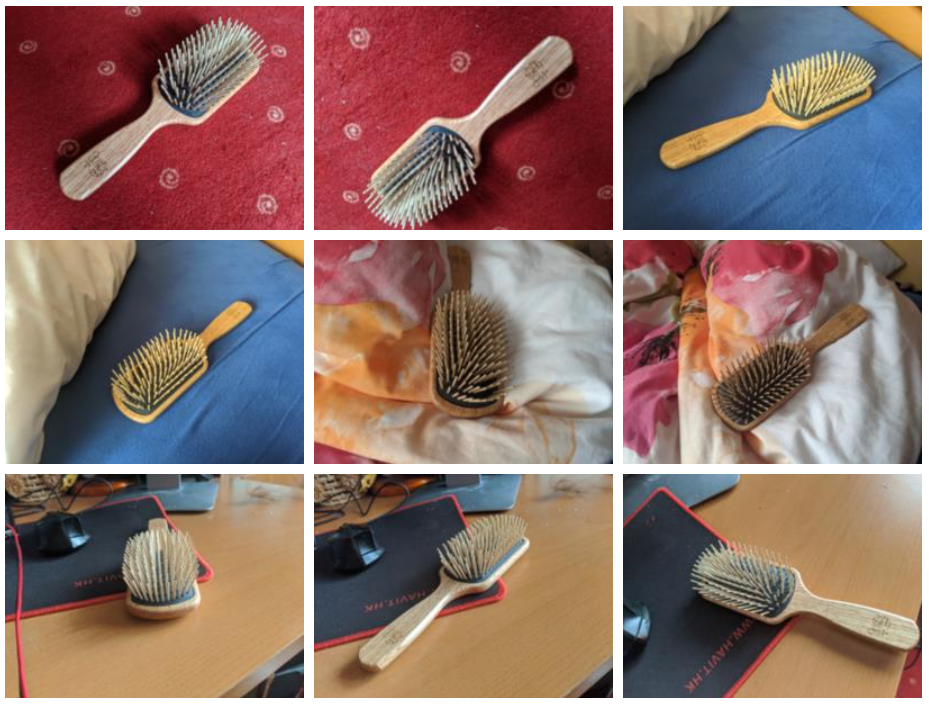
\includegraphics[width=0.8\textwidth]{images/img_it4train.PNG}
	\caption[Ausschnitt der Trainigsbilder. Iteration 4]{Ausschnitt der Trainigsbilder für Haarbürsten-Objekterkennung Iteration 4}
	\label{img:it4training}
\end{figure}

\begin{figure}[H]
	\centering
	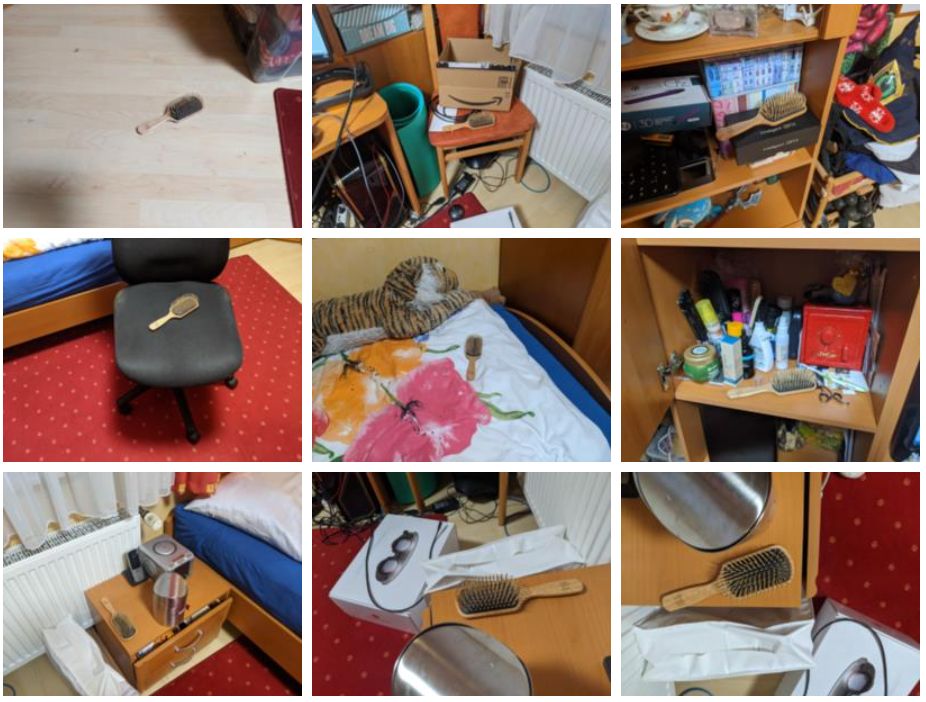
\includegraphics[width=0.8\textwidth]{images/img_it6train.PNG}
	\caption[Ausschnitt der Trainigsbilder. Iteration 6]{Ausschnitt der Trainigsbilder für Haarbürsten-Objekterkennung Iteration 4}
	\label{img:it6training}
\end{figure}

\subsection{Beispielbilder von Objekten mit Labeln}
\label{appendix:bsp}

\begin{figure}[H]
	\centering
	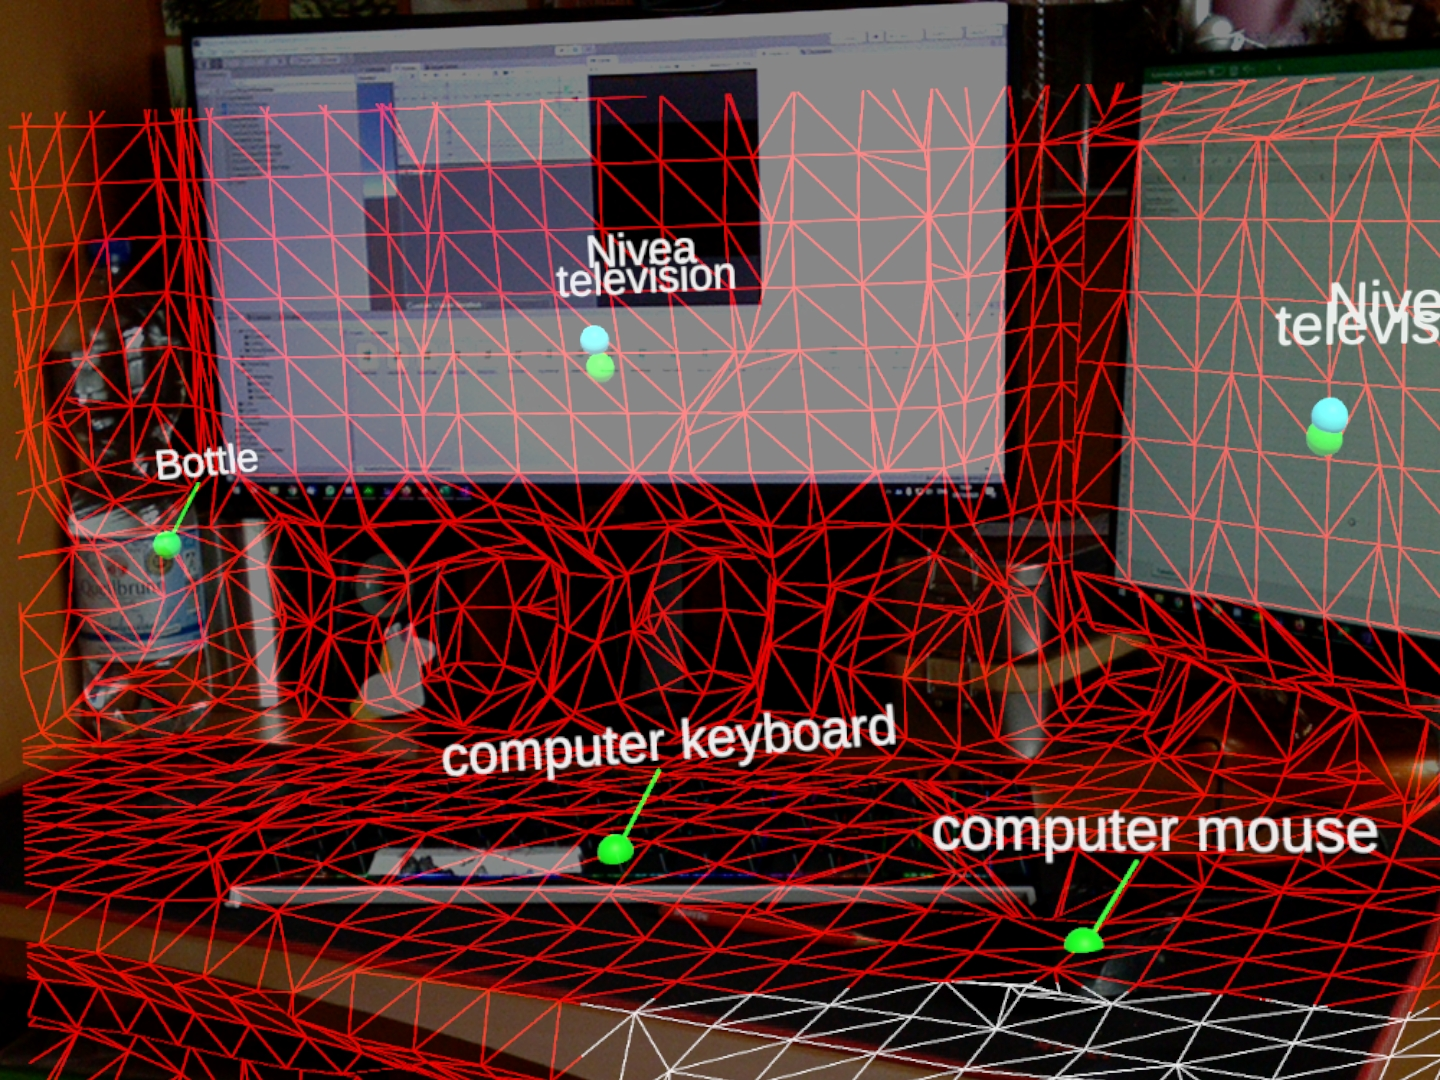
\includegraphics[width=0.8\textwidth]{images/ML_20201005_15.28.37.jpg}
	\caption[Beispielbild mit Iteration 4.]{Beispielbild mit Iteration 4. Computerbildschirme werden als Nivea Dosen erkannt.}
\end{figure}

\begin{figure}[H]
	\centering
	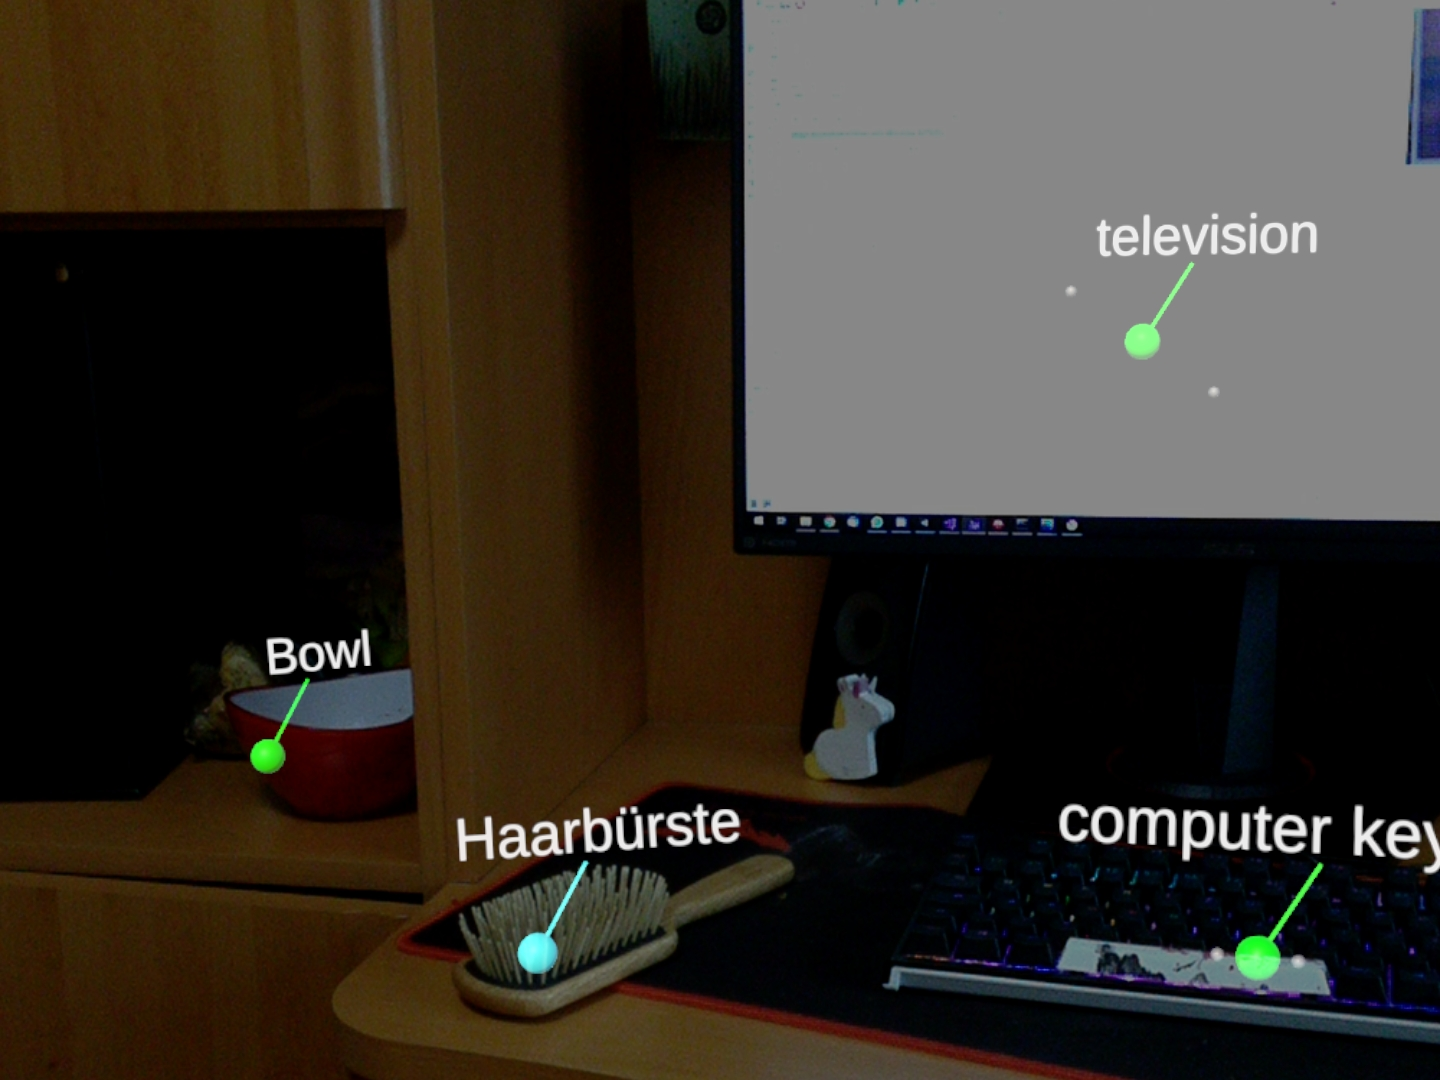
\includegraphics[width=0.8\textwidth]{images/ML_20201014_13.05.56.jpg}
	\caption[Beispielbild mit Iteration 6.]{Beispielbild mit Iteration 6}
\end{figure}

